\mychapter{Límits i continuïtat}{Límits i continuïtat}{
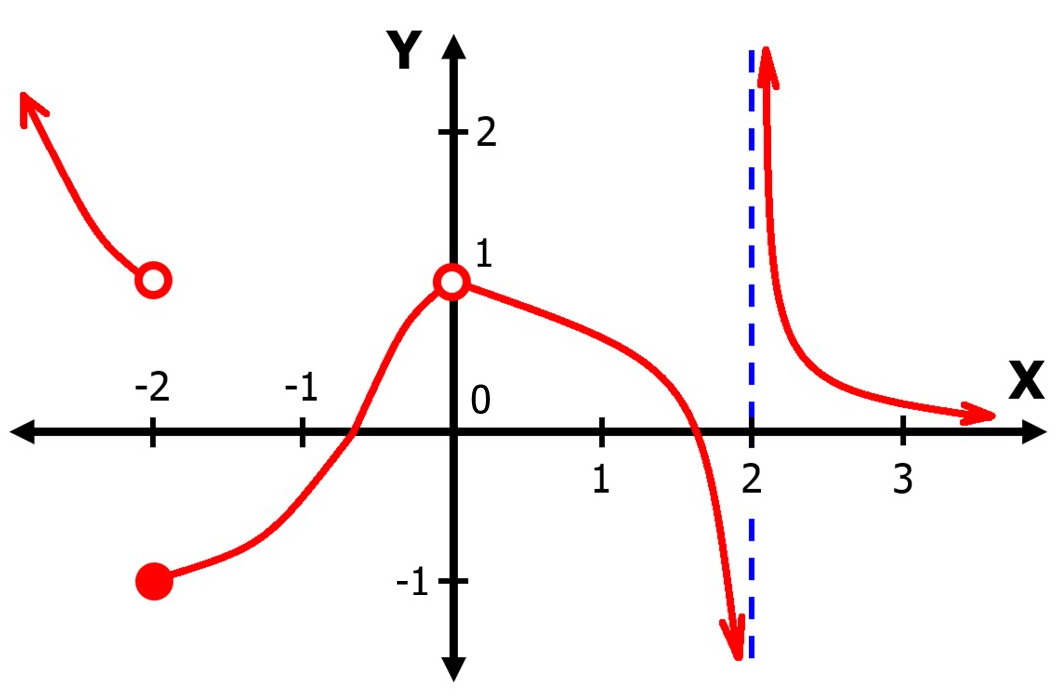
\includegraphics[width=4.5cm]{img-06/chap7.png}}{chap:limits}


\section{Concepte de límit}

\begin{blueshaded}
	\begin{itemize}
		 
	\item Direm que \textbf{$x$ tendeix a $a$ per la dreta} ($x \to a^+$) si $x$ pren valors majors que $a$ i cada vegada més propers a ell,
	
	\quad $x \to 3^+$ \quad si \quad $x=$3.1, 3.01, 3.001, $\cdots$.
	
	\item Direm que $x$ \textbf{tendeix a $a$ per l'esquerra} ($x \to a^-$) si $x$ pren valors menors que $a$ i cada vegada més propers a ell,
	
	\quad $x \to 3^-$ \quad si \quad $x=$2.9, 2.99, 2.999, $\cdots$.
	
	\item Direm que $x$ \textbf{tendeix a $a$}  ($x \to a$) si $x$ pren valors  cada vegada més propers a $a$,
	
	\quad $x \to 3$ \quad si \quad $x=$3.1, 2.99, 3.001, $\cdots$.

\item Direm que $x$ \textbf{tendeix a $+\infty$}  ($x \to +\infty$) si $x$ pren valors positius cada vegada més grans,

\quad $x \to  +\infty$ \quad si \quad $x=$10, 1000, 1000000, $\cdots$.

\item Direm que $x$ \textbf{tendeix a $-\infty$ } ($x \to -\infty$) si $x$ pren valors negatius cada vegada més grans,

\quad $x \to -\infty$ \quad si \quad $x=-$10, $-$1000, $-$1000000, $\cdots$.
	\end{itemize}
\end{blueshaded}

\begin{theorybox}
 
	  Direm que el límit d'una funció en un punt existeix si els dos \textbf{límits laterals coincideixen}, és a dir
	  
	  \begin{equation*}
	  \limx{a^-} f(x) = \limx{a^+} f(x) = \limx{a} f(x)
	  \end{equation*}
\end{theorybox}

\pagebreak

\begin{mylist}
	
	\exer Per a cadascuna de les funcions següents $f_1(x)=\dfrac{-5}{(x-3)^2}$, $f_2(x)=\dfrac{4}{3-x}$, \linebreak $f_3(x)=2^x$, completa en el teu quadern la taula adjunta, amb l'ajuda de la calculadora, i estima el valor de $\limx{3^-} f(x)$.
	
	\begin{center}
		\begin{tabular}{|c|c|c|c|c|c|}
			\hline
			$x$ & 2 & 2,5 & 2,9 & 2,99 & 2,999 \\ \hline
			$f(x)$ & & & & & \\ \hline
		\end{tabular}
	\end{center}

\answers{$\limx{3^-} f_1(x)=-\infty$\par
\begin{tabular}{|c|c|c|c|c|c|}
	\hline
	$x$ & 2 & 2,5 & 2,9 & 2,99 & 2,999 \\ \hline
	$f_1$ & -5 & -20 & -500 & $-5\cdot 10^4$&  $-5\cdot 10^6$\\ \hline
\end{tabular}\par
%%
$\limx{3^-} f_2(x)=+\infty$\par
\begin{tabular}{|c|c|c|c|c|c|}
	\hline
	$x$ & 2 & 2,5 & 2,9 & 2,99 & 2,999 \\ \hline
	$f_2$ & 4 & 8& 40& 400& 4000 \\ \hline
\end{tabular}\par
%%
$\limx{3^-} f_3(x)=8$\par
\begin{tabular}{|c|c|c|c|c|c|}
	\hline
	$x$ & 2 & 2,5 & 2,9 & 2,99 & 2,999 \\ \hline
	$f_3$ & 4 & 5,66 & 7,46 & 7,94 & 7,99 \\ \hline
\end{tabular}
}


\exer Observant cadascuna de les gràfiques següents
\begin{center}
	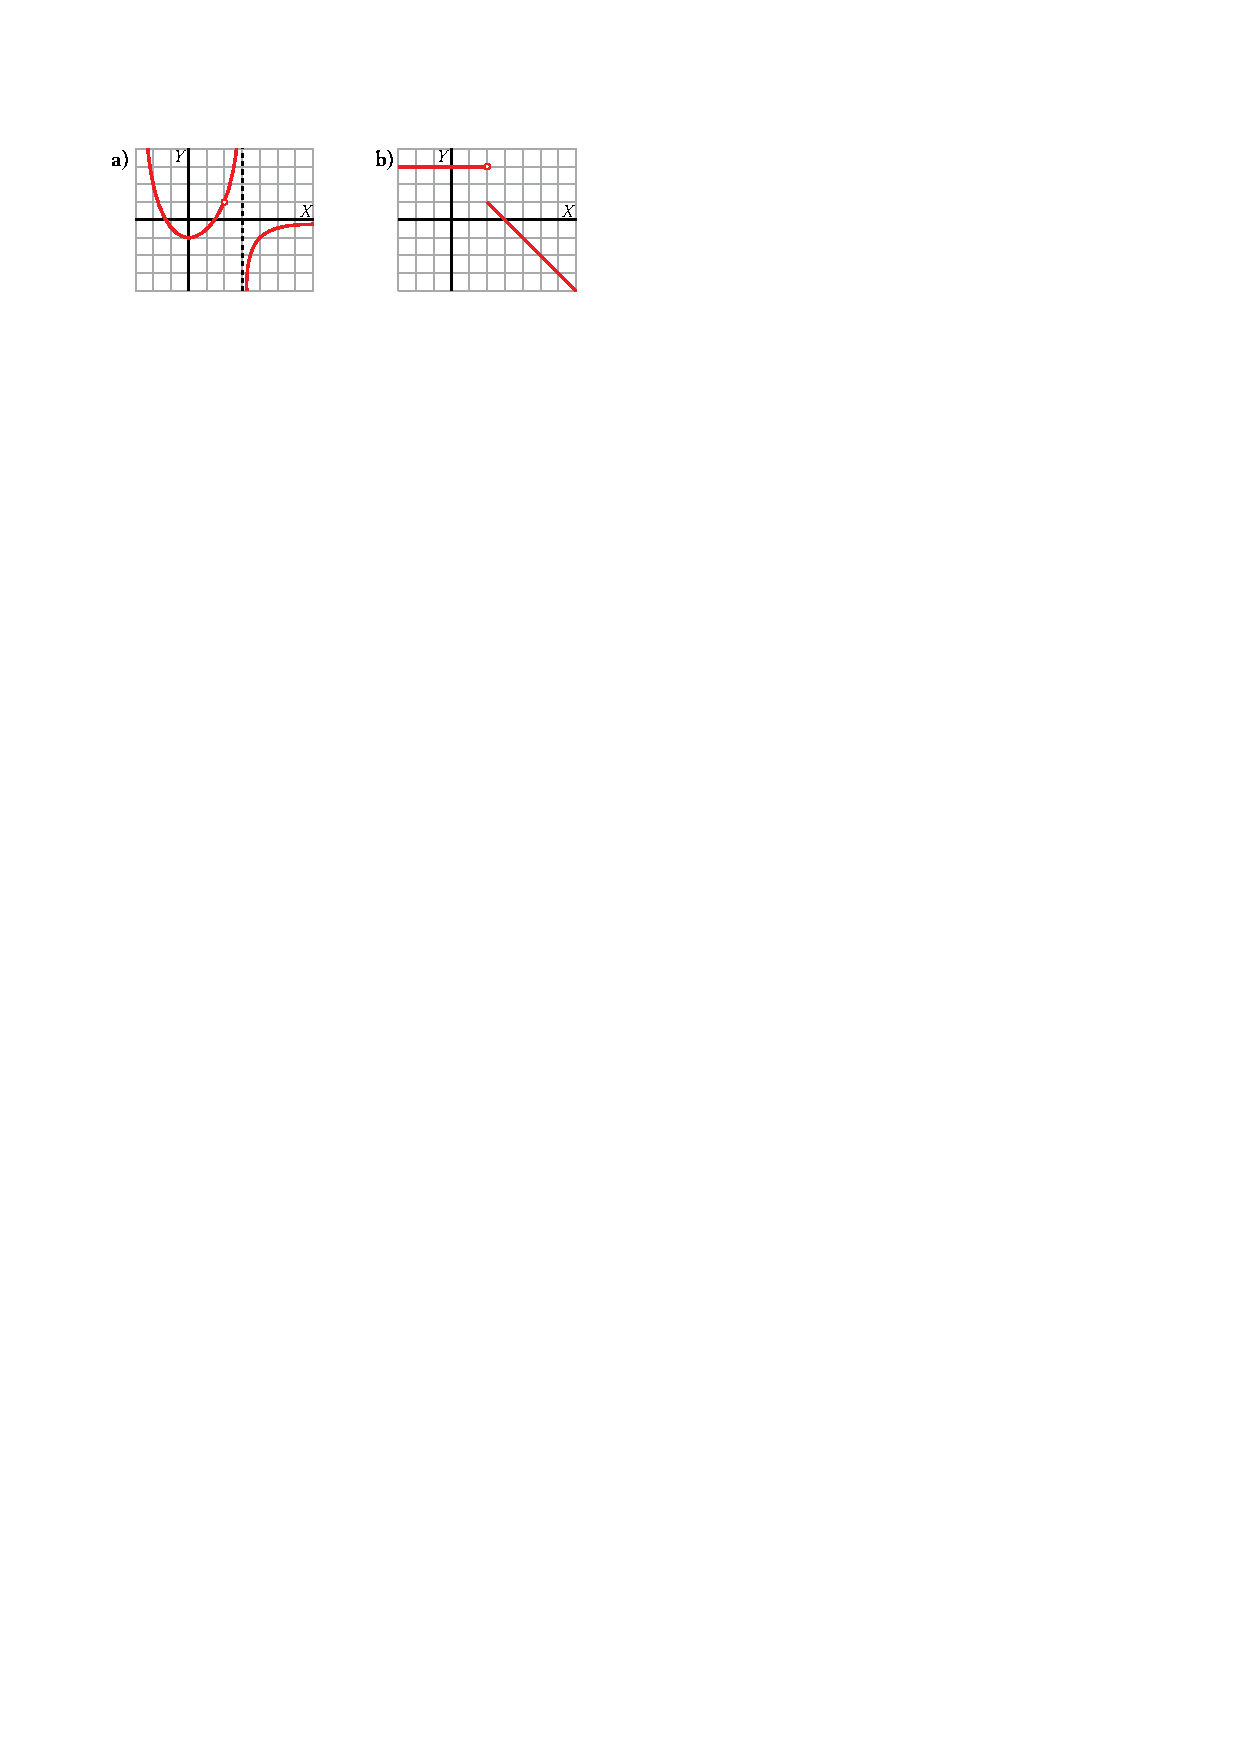
\includegraphics[width=10cm]{img-06/limits1.pdf}
\end{center}
troba $\limx{3} f(x)$, $\limx{2} f(x)$, $\limx{+\infty} f(x)$, $\limx{-\infty} f(x)$.

\answers[cols=1]{[
	 $\limx{3} f(x)=\nexists$; $\limx{2} f(x)=1$; $\limx{+\infty} f(x)=0^-$; $\limx{-\infty} f(x)=+\infty$,
	 $\limx{3} f(x)=0$; $\limx{2} f(x)=\nexists$; $\limx{+\infty} f(x)=-\infty$; $\limx{-\infty} f(x)=3$
	]}


\exer  Calcula els límits laterals i determina si existeix el límit en les funcions següents definides a trossos, en els punts en els quals s'uneixen dues branques:


\begin{tasks}(2) 	
	\task $f(x)=\left\{\begin{array}{cc} {-2x+3} & {si\; x<1} \\ {3x-2} & {si\; x\ge 1} \end{array}\right. $   
	\task $f(x)=\left\{\begin{array}{cc} {\dfrac{-2x+3}{x+5} } & {si\; x<1} \\ [0.4cm] {\dfrac{5x^{2} }{x+3} } & {si\; x\ge 1} \end{array}\right. $  
	\task $f(x)=\left\{\begin{array}{cc} {\dfrac{1}{x} } & {si\; x<0} \\ [0.4cm] {\dfrac{x}{x+1 } } & {si\; x\ge 0} \end{array}\right. $ 
	\task $f(x)=\left\{\begin{array}{cc} {\dfrac{x^2-25}{x-5} } & {si\; x<5} \\ [0.4cm] {x+5 } & {si\; x\ge 5} \end{array}\right. $ 
\end{tasks}

\answers{[$\limx{1^-} f=1$; $\limx{1^+} f=1$,
	$\limx{1^-} f=1/6$; $\limx{1^+} f=5/4$,
	$\limx{0^-} f=-\infty$; $\limx{0^+} f=0$,
	$\limx{5^-} f=10$; $\limx{5^+} f=10$]}  

\end{mylist}




\section{Càlcul de límits}

\begin{theorybox}
	Recorda: Podem classificar els límits en un punt en:
	\begin{itemize}
		\exer \textbf{Immediats:} Només cal substituir el valor de $x$ dins la funció.
		\exer \textbf{Infinits:} Quan substituïm valor de $x$ dins la funció, trobam una divisió per zero $\dfrac{k}{0}$. El límit pot donar $\pm \infty$. Cal calcular els dos límits laterals.
			\exer \textbf{Indeterminats:} Una indeterminació és una expressió que no sabem el seu valor si no feim alguna cosa més. Cada tipus d'indeterminació té una tècnica per descobrir el seu valor.
			
			Són indeterminacions expressions com ara:
		     \begin{center}
			$0/0$, \quad $\infty/\infty$, \quad $\infty - \infty$,\quad  $0\cdot \infty$,\quad  $1^\infty$, ...
			\end{center}
		
	\end{itemize}
\end{theorybox}

\vspace{2cm} 
\subsection{Límits a un punt}

\begin{theorybox}
	\videonw{173}{Límits de funcions racionals en un punt.}
\end{theorybox}
 
\begin{resolt}[E]{Calcula els límits  de la funció 
	\begin{equation*}
		f(x)=\dfrac{x+3}{x^{2} -9}
	\end{equation*}
quan \vspace{0.25cm}

\quad a) $x\rightarrow 1$

\quad b) $x\rightarrow 3$

\quad c) $x\rightarrow -3$
}

 a) Immediat: 
  $\limx{1} \dfrac{x+3}{x^{2} -9} = \dfrac{1+3}{1-9} = - \dfrac{1}{2} $ \vspace{0.75cm}
 
 b) Infinit:  $\limx{3} \dfrac{x+3}{x^{2} -9} = \dfrac{6}{0} = \left\{ \begin{array}{l} 
 	 \limx{3^-} \dfrac{x+3}{x^{2} -9}  = \dfrac{+6}{-0} = -\infty \\  \limx{3^+} \dfrac{x+3}{x^{2} -9}  = \dfrac{+6}{+0} = +\infty
 \end{array} \right.$ \vspace{0.75cm}
	
 c) Indeterminació 0/0:
  $\limx{-3} \dfrac{x+3}{x^{2} -9} = \dfrac{0}{0} = \mathrm{IND}=$\par \qquad   $=\limx{-3} \dfrac{(x+3)}{(x+3)\cdot (x-3)}= \limx{-3} \dfrac{1}{x-3}= -\dfrac{1}{6} $ 
 
 
\end{resolt}







\begin{mylist}
	
	\exer  Calcula els següents límits, indicant el signe:
	\begin{tasks}(4) 
		\task  $\limx{1^{+} } \dfrac{5}{x-1} $ \task  $\limx{1^{-} } \dfrac{5}{x-1} $  \task  $\limx{3^{+} } \dfrac{-5}{x-3} $  \task $\limx{3^{-} } \dfrac{-5}{x-3} $
	\end{tasks}
	\answers{[$+\infty$, $-\infty$, $-\infty$, $+\infty$]}
\vso	

\exer[1] Calcula els límits següents
\begin{tasks}(4) 
	\task  $\limx{-3} \dfrac{x+3}{x^{2} -9} $   \task $\limx{-3} \dfrac{x^{2} -9}{x-3} $   \task $\limx{-3} \dfrac{x^{3} +27}{x^{2} +3x} $   \task $\limx{1} \dfrac{x^{3} -1}{x^{2} +x-2} $
	\task $\limx{-2} \dfrac{x^{3} +8}{-x-2} $   \task $\limx{1} \dfrac{\sqrt{3+x} -4}{x-1} $  \task $\limx{-4} \dfrac{x^{3} +8x-2}{-x^{2} -2x+3} $
\end{tasks}
\answers{[--1/6, 0, --9, 1, --12, $\mp\infty$, 98/5]}

\vso	
\exer[1] Calcula els límits següents
\begin{tasks}(3) 
	\task $\limx{3} \left(\dfrac{1}{x^2-9} - \dfrac{1}{x-3} \right)$
	\task $\limx{1} \left(\dfrac{2}{x^2-1} - \dfrac{1}{x-1} \right)$
	\task $\limx{3} \left(\dfrac{x^2 -5x+6}{x^2-9} \right)$
	\task $\limx{1} \left(\dfrac{x^3-4x^2+4}{(x-1)^2}  \right)$
	\task $\limx[h]{0} \left(\dfrac{\sqrt{3-h} - \sqrt{3}}{h} \right)$
	\task $\limx{2} \left(\dfrac{2 - \sqrt{2+x}}{x-2} \right)$
\end{tasks}
\answers{[$\infty$, --1/2, 1/6, $+\infty$, $-1/(2\sqrt{3})$, --1/4]}

\end{mylist}

\pagebreak
\begin{center}
	
	\heading{Regles bàsiques pel càlcul de límits}
	
	\setlength\LTleft{0pt}
	\setlength\LTright{0pt}
	\fontsize{10.5}{11}
	\def\arraystretch{1.8}
	\begin{longtable}[h]{|p{0.22\textwidth}|p{0.27\textwidth}|p{0.45\textwidth}|}
		\hline
		\multicolumn{3}{|c|}{Me demanen $\limx{a} f(x)$} \\  [1.5ex] \hline  
		\cellcolor{lightgray} \textit{Quan substutueixo $x$ per $a$ trob}  & \cellcolor{lightgray} \textit{Què faré?} & \cellcolor{lightgray} \textit{Exemple} \\  [1.5ex] \hline  
		Un nombre & Res. Ja he acabat! & $\limx{2} x^2=2^2=4$\\  [1.5ex] \hline  
		$\dfrac{k}{0}$ & Calcular els límits laterals per saber si val $\pm \infty$ & $\limx{2} \dfrac{1}{x-2}=\left\{\begin{array}{l} \limx{2^-} \dfrac{1}{x-2}=-\infty \\  \limx{2^+} \dfrac{1}{x-2}=+\infty \end{array}\right .$ \\[1.5ex] \hline  
		$\dfrac{0}{0}$ amb polinomis & Factoritzar i simplificar & $\limx{5} \dfrac{x^2-25}{x-5}=\limx{5} \dfrac{(x+5)(x-5)}{(x-5)}=\limx{5} (x+5)=10$  \\  [1.5ex] \hline  
		$\dfrac{0}{0}$ amb arrels & Racionalitzar i simplificar & $\limx{3} \dfrac{\sqrt{x+6}-3}{x-3}=\limx{3} \dfrac{(\sqrt{x+6}-3)\cdot(\sqrt{x+6}+3)}{(x-3)\cdot(\sqrt{x+6}+3)}=\cdots=\dfrac{1}{6}$ \\  [1.5ex] \hline  
	\end{longtable}
\end{center}

 \begin{center}
 	\setlength\LTleft{0pt}
 	\setlength\LTright{0pt}
 	\fontsize{10.5}{11}
 	\def\arraystretch{1.8}
 	\begin{longtable}[h]{|p{0.22\textwidth}|p{0.27\textwidth}|p{0.45\textwidth}|}
 		\hline
 		\multicolumn{3}{|c|}{Me demanen $\limx{\pm \infty} f(x)$} \\  [1.5ex] \hline  
 		\cellcolor{lightgray}\textit{Quan substitueixo $x$ per $\pm \infty$ trob}  & \cellcolor{lightgray}\textit{Què faré?} & \cellcolor{lightgray}\textit{Exemple}\\  [1.5ex] \hline  
 		$\dfrac{k}{\infty}$ & El límit val 0. & $\limx{\infty} \dfrac{5}{x^2}=0$\\  [1.5ex] \hline  
 		$\dfrac{\infty}{\infty}$ amb polinomis & Dividim tot per la major potència de $x$ del denominador. & $\limx{\infty} \dfrac{2x^2+5}{3x^2-2x+1}=$ dividim per $x^2$ $=\limx{\infty} \dfrac{2+5/x^2}{3-2/x+1/x^2}=\dfrac{2}{3}$\\  [1.5ex] \hline  
 		$\dfrac{\infty}{\infty}$  amb arrels & El mateix que abans, però ara l'exponent dins d'una arrel queda dividit entre 2. & $\limx{\infty} \dfrac{2x+5}{\sqrt{3x^2-2x+1}}=$ dividim per $x$ $=\limx{\infty} \dfrac{2+5/x}{\sqrt{3-2/x+1/x^2}}=\dfrac{2}{\sqrt{3}}$\\  [1.5ex] \hline  
 		$\infty - \infty$  amb polinomis & Calcular el mcm i operar les fraccions & $\limx{\infty} \dfrac{x^2}{x+1}-x=\cdots=\limx{\infty} \dfrac{-x}{x+1}=-1$\\  [1.5ex] \hline  
 		$\infty - \infty$  amb arrels & Racionalitzar i simplificar & $\limx{\infty} \sqrt{x^2-1}-x=$ 
 		
 		$\limx{\infty} (\sqrt{x^2-1}-x)\dfrac{(\sqrt{x^2-1}+x)}{(\sqrt{x^2-1}+x)}=\cdots=0$ \\[1.5ex] \hline  
 	\end{longtable}
 \end{center}

 \pagebreak
\subsection{Límits a l'infinit}


\begin{theorybox}
	\begin{minipage}{0.5\textwidth}
		\centering
		\videonw{174}{Com calcular límits de polinomis a l'infinit?}
	\end{minipage}
	\begin{minipage}{0.5\textwidth}
		\centering
		\videonw{175}{Com calcular límits de funcions racionals a l'infinit?}
	\end{minipage}
	
	
\end{theorybox}

\begin{mylist}
	
		\exer \mental Classifica els següents límits en finits o infinits, i calcula'ls:
	\begin{tasks}(4) 
		\task  $\limx{\infty } -x^{2} $  \task  $\limx{\infty } +x^{2} $   \task  $\limx{3} x^{2} $  \task  $\limx{\infty } \dfrac{1}{x^{2} } $
	\end{tasks}
\answers{[$-\infty$, $+\infty$, $9$, $0$]}

	\exer  Calcula els següents límits, indicant el signe:
	\begin{tasks}(3) 
		\task  $\limx{+\infty } -x^{3}+2x^2+5 $ \task  $\limx{-\infty } -x^{3}-7x+5 $   \task  $\limx{\infty } x^{2}+x-4 $ \task  $\limx{+\infty } \dfrac{1}{x^{2} } $   \task  $\limx{-\infty } \dfrac{1}{x^{2} - 5x + 4 } $
	\end{tasks}
\answers{[$-\infty$, $+\infty$, $+\infty$, 0, 0]}

\end{mylist}

\begin{theorybox}
	Els límits de les funcions racionals a l'infinit segons els grau del numerador $D(x)$ i denominador $d(x)$  poden valer: 
	\begin{equation*}
	\limx{\infty} \dfrac{D(x)}{d(x)} = \left\{ \begin{array}{ll} 0 & \mathrm{grau}\, D < \mathrm{grau}\, d \\ L & \mathrm{grau}\, D = \mathrm{grau}\, d \\ \pm\infty & \mathrm{grau}\, D > \mathrm{grau}\, d \end{array} \right.
\end{equation*}
\end{theorybox}

\begin{mylist}
	\exer Escriu, sense necessitat de fer càlculs, el valor dels límits següents:

	\begin{tasks}(2) 
		\task  $\limx{+\infty} \dfrac{5x^2+3}{5x^2+2x-1}$
		\task  $\limx{+\infty} \dfrac{5x^5+3}{5x^2+2x-1}$
		\task  $\limx{+\infty} \dfrac{5x^2+3}{5x^7+2x-1}$
		\task  $\limx{+\infty} \dfrac{4x^3+3x^2-2x+5}{2x^3+x^2-x}$	
	\end{tasks}

	\answers{[$1$, $+\infty$, $0$, $2$]}
	
	\exer[1] Calcula els límits següents
	
	\begin{tasks}(2) 
		\task $\limx{\infty } \dfrac{x^{3} +8}{-x-2} $ 
		\task $\limx{\infty } \dfrac{x^{3} +8}{-x^{5} -2} $   
		\task $\limx{\infty } \dfrac{3x^{3} +8}{-x^{3} -2} $   
		\task $\limx{\infty } \left(\dfrac{3x}{x^{2} -4} -\dfrac{2}{x+2} \right)$
	\task $\limx{\infty } \left(\dfrac{3x}{x^{2} -4} -\dfrac{x-3}{x+2} \right)$  
	 \task $\limx{\infty } \left(\sqrt{3x-1} -\sqrt{x^{2} -2x} \right)$  
	 \task $\limx{\infty } \left(\sqrt{x-1} -\sqrt{x-2} \right)$ 
	 \task $\limx{\infty } \left(\dfrac{1}{\sqrt{x-2} -\sqrt{x+2} } \right)$
	\end{tasks}
	\answers{[$-\infty$, 0, $-3$, 0, $-1$, $-\infty$, $0$, $-\infty$]}

\end{mylist}
\pagebreak

\begin{warningbox}
	
	El número $e$ s'obté del límit
	\[ \limx[n]{\infty} \left( 1+ \frac{1}{n} \right)^n = e \approx 2.718281828459045 \]
	
	Totes les indeterminacions del tipus $1^\infty$ estan relacionades amb el número $e$.
	
\end{warningbox}

\begin{theorybox}
	Els límits de les funcions exponencials a l'infinit segons la base, quan l'exponent $h(x) \rightarrow +\infty$ poden valer: 
	\begin{equation*}
	\limx{\infty} \left(\dfrac{f(x)}{g(x)}\right)^{h(x)} = \left\{ \begin{array}{ll} 0 & \mathrm{si}\,\, 	\limx{\infty} \dfrac{f(x)}{g(x)}<1 \\ e^{\limx{\infty} h(x)\cdot\left( \frac{f(x)}{g(x)} -1 \right)} & \mathrm{si}\,\, 	\limx{\infty} \dfrac{f(x)}{g(x)}=1  \\ \infty & \mathrm{si}\,\, 	\limx{\infty} \dfrac{f(x)}{g(x)}>1 \end{array} \right.
	\end{equation*}
\end{theorybox}

\begin{mylist}
	
	
	\exer Determina els límits següents:
	\begin{tasks}(4)
		\task  $\limx{+\infty} 2^x$
		\task  $\limx{+\infty} \left(\dfrac{1}{2}\right)^x$
		\task  $\limx{+\infty} 2^{-x}$	
		\task  $\limx{+\infty} 10^{\frac{1}{x}}$
	    \task  $\limx{+\infty} 10^{\frac{x^2+1}{x}}$
		\task  $\limx{+\infty} e^{\frac{2x-1}{x+1}}$
		\task  $\limx{+\infty} 5^{2x^2-1}$			
	\end{tasks}	
\answers{[$+\infty$, $0$, $0$, $1$, $+\infty$, $e^2$, $+\infty$]}
	
	\exer Determina els límits següents:
		\begin{tasks}(3) 
		\task  $\limx{+\infty} \left( \dfrac{x+1 }{x-2 } \right) ^{2x^2-1}$
		\task  $\limx{+\infty} \left( \dfrac{x^3-1 }{x^3+5 } \right) ^{3x^2}$
		\task  $\limx{+\infty} \left( \dfrac{3x^3+x }{3x^2-2 } \right) ^{\frac{2x^2-1}{x^3}}$
%		\task  $\limx{+\infty} \left( \dfrac{5x+3 }{5x^2+1 } \right) ^{\frac{x^2-1}{5x^3}}$
%		\task  $\limx{+\infty} \left( \dfrac{5x+3 }{5x+1 } \right) ^{\frac{x^2-1}{5x}}$
%		\task  $\limx{+\infty} \left( \dfrac{5x+3 }{x+2 } \right) ^{\frac{x^2-1}{5x}}$
%		\task  $\limx{+\infty} \left( \dfrac{ x^3-1 }{ 4x^3+5 } \right) ^{3x^2}$
%		\task  $\limx{+\infty} \left( \dfrac{3x^2+x }{3x^2-2 } \right) ^{\frac{2x^2-1}{x}}$
      	\end{tasks}
      \answers{[$+\infty$, $1$, $1$]}
	
\end{mylist}


\subsection{Fitxa de límits}

\begin{mylist}
	\exer[1] Calcula els següents límits utilitzant les tècniques adequades en cada cas

\begin{tasks}[counter-format=(tsk[1]),label-width=4ex](2)
\task $\limx{0 } \dfrac{x^2-x}{x^2}$
\task $\limx{0 } \dfrac{x^3-3x^2}{2x^2}$
\task $\limx{2 } \dfrac{2-x}{x^2-4}$
\task $\limx{1/2 } \dfrac{x+1}{2x-1}$
\task $\limx{-1 } \dfrac{x^2+2x+1}{x^2+8x+7}$
\task $\limx{-7} \dfrac{x^2+2x+1}{x^2+8x+7}$
\task $\limx{-2 } \dfrac{x-3}{x^2-4}$
\task $\limx{4 } \dfrac{2x-3}{(x-4)^2}$
\task $\limx{1 } \dfrac{3x}{x-1}$
\task $\limx{5 } \dfrac{x^2-25}{x-5}$
\task $\limx{5 } \dfrac{x^2-25}{x^2-10x+25}$
\task $\limx{1 } \dfrac{x^4-3x^3-3x^2+11x-6}{x^3-4x^2+5x-2}$
\task $\limx{+\infty } (3x-5)$
\task $\limx{+\infty } (-3x+7)$
\task $\limx{-\infty } (6x^2-10x+17)$
\task $\limx{+\infty } \dfrac{1}{x}$
\task $\limx{-\infty } \dfrac{-14}{x^2}$
\task $\limx{\pm\infty } \dfrac{3}{x-5}$
\task $\limx{+\infty } \dfrac{2x+3}{x^2-4x+1}$
\task $\limx{+\infty } \dfrac{2x^2+3x}{5x^2-4x+1}$
\task $\limx{-\infty } \dfrac{-7x^2+3x}{3x^2-4x+1}$
\task $\limx{+\infty } \dfrac{x^2-2x}{2x+7}$
\task $\limx{+\infty } \dfrac{-3x^2+8x}{x-4}$
\task $\limx{-\infty } \dfrac{-3x^2+8x}{x-4}$
\task $\limx{3\pi /2 } \sin x$
\task $\limx{\pi /2 } \mathrm{tg}\, x$
\task $\limx{0^+} \log_2 x$
\task $\limx{0 } \sqrt{\dfrac{x^2-2x+3}{x+1}}$
\task $\limx{-\infty } \dfrac{x^2+5x+7}{2x^2+x+1}$
\task $\limx{-\infty } \dfrac{-x^2+3x+21}{5x^2-4x^3+2x}$
\task $\limx{+\infty } \dfrac{x^3-2x^2-10x}{-x^2+5x^3-x+3}$
\task $\limx{-\infty } \dfrac{4+x-2x^3}{2x^2-3x+11}$
\task $\limx{\infty } \left( \dfrac{x^2}{x-2} - \dfrac{2x^2-3x+1}{2(x-2)} \right)$
\task $\limx{+\infty } \dfrac{2x+3}{\sqrt{x^2-4x+1}}$
\task $\limx{+\infty } \dfrac{2x-4}{\sqrt{2x^3-4x}}$
\task $\limx{+\infty } \dfrac{2x^2}{\sqrt{x^3+2x}}$
\task $\limx{4 } \dfrac{\sqrt{x}-2}{\sqrt{x-4}}$
\task $\limx{2 } \dfrac{2-\sqrt{x}}{2x-4}$
\task $\limx{2 } \dfrac{2x-4}{\sqrt{2-\sqrt{2x}}}$
\task $\limx{3 } \dfrac{\sqrt{2x+3}-x}{3-x}$
\task $\limx{3 } \dfrac{2x-\sqrt{4x-3}}{x^2-9}$
\task $\limx{+\infty } \left( \sqrt{4x^2+2x} - \sqrt{4x^2-3} \right)$
\end{tasks}
\answers{\begin{tasks}[counter-format=(tsk[1]),label-width=4ex](2)
		\task*(2) $\mathop{lim}\limits_{x\to 0^- } f(x)=+\infty$, $\mathop{lim}\limits_{x\to 0^+ } f(x)=-\infty$
		\task $-3/2$
		\task $-1/4$\startnewitemline
		\task*(2) $\mathop{lim}\limits_{x\to 1/2^- } f=-\infty$, $\mathop{lim}\limits_{x\to 1/2^+ } f=+\infty$
		\task 0\startnewitemline
		\task*(3) $\mathop{lim}\limits_{x\to 7^- } f(x)=+\infty$, $\mathop{lim}\limits_{x\to 7^+ } f(x)=-\infty$
		\task*(2)  $\mathop{lim}\limits_{x\to 2^- } f(x)=-\infty$, $\mathop{lim}\limits_{x\to 2^+ } f(x)=+\infty$
		\task $+\infty$\startnewitemline
		\task*(2)  $\mathop{lim}\limits_{x\to 1^- } f(x)=-\infty$, $\mathop{lim}\limits_{x\to 1^+ } f(x)=+\infty$
		\task 10\startnewitemline
		\task*(2) $\mathop{lim}\limits_{x\to 5^- } f(x)=-\infty$, $\mathop{lim}\limits_{x\to 5^+ } f(x)=+\infty$
		\task 6
		\task $+\infty$
		\task $-\infty$
		\task $+\infty$
		\task $0$
		\task $0$
		\task $0$
		\task $0$
		\task $2/5$
		\task $-7/3$
		\task $+\infty$
		\task $-\infty$
		\task $+\infty$
		\task $-1$
		\task*(2)  $\mathop{lim}\limits_{x\to 0^- } f(x)=+\infty$, $\mathop{lim}\limits_{x\to 0^+ } f(x)=-\infty$
		\task $-\infty$
		\task $\sqrt{3}$
		\task 1/2
		\task 0
		\task 1/5
		\task $+\infty$
		\task 3/2
		\task 2
		\task 0
		\task $+\infty$
		\task $1/4$\startnewitemline
		\task*(2)  $\mathop{lim}\limits_{x\to 2^- } f(x)=-\infty$, $\mathop{lim}\limits_{x\to 2^+ } f(x)=+\infty$
		\task -4
		\task 2/3\startnewitemline
		\task*(2)  $\mathop{lim}\limits_{x\to 3^- } f(x)=-\infty$, $\mathop{lim}\limits_{x\to 3^+ } f(x)=+\infty$
		\task 1/2
\end{tasks}}
	
\begin{comment}
\vspace{2cm}
\exer[1] Calcula els següents límits utilitzant les tècniques adequades en cada cas
\begin{tasks}[counter-format=(tsk[1]),label-width=4ex](2)
	\task $\mathop{lim}\limits_{x\to 5 } \dfrac{x-\sqrt{3x+10}}{x^2-25}$
	\task $\mathop{lim}\limits_{x\to 0 } \left( \dfrac{x+1}{6x^2} -   \dfrac{2x+3}{3x^3} \right)$
	\task $\mathop{lim}\limits_{x\to 1 } \left( \dfrac{2x+3}{x^2-1} : \dfrac{2x+2}{x-1} \right)$
	\task $\mathop{lim}\limits_{x\to -1 } \dfrac{x^2+2x+1}{x^3+3x^2+3x+1}$
	\task $\mathop{lim}\limits_{x\to 1 } \dfrac{x^2+x-2}{x^2+5x+6}$
	\task $\mathop{lim}\limits_{x\to -2 } \dfrac{3x^2-9x-30}{16+2x^3}$
	\task $\mathop{lim}\limits_{x\to 3 } \dfrac{x^3-2x^2-3x}{27-x^3}$
	\task $\mathop{lim}\limits_{x\to -3 } \dfrac{3x+9}{x^3-27}$
	\task $\mathop{lim}\limits_{x\to \infty } \dfrac{2-x-5x^2}{3x^2+1}$
	\task $\mathop{lim}\limits_{x\to \infty } \dfrac{7x-3}{4x^2+2}$
	\task $\mathop{lim}\limits_{x\to \infty } \left( \sqrt{x^2+1}-x-2 \right)$
	\task $\mathop{lim}\limits_{x\to -\infty } \left( 3x^3 + 2 - \sqrt{5x^4-3x^2+7} \right)$
	\task $\mathop{lim}\limits_{x\to -\infty } \dfrac{1-3x^3}{5x^2+2}$
\end{tasks}
\answers{\begin{tasks}[counter-format=(tsk[1]),label-width=4ex](2)
		\task 7/100
		\task*(2) Laterals  $\mathop{lim}\limits_{x\to 0^- } f(x)=+\infty$, $\mathop{lim}\limits_{x\to 0^+ } f(x)=-\infty$
		\task 5/8
		\task*(2) Laterals  $\mathop{lim}\limits_{x\to -1^- } f(x)=-\infty$, $\mathop{lim}\limits_{x\to -1^+ } f(x)=+\infty$
		\task 0
		\task $-7/8$
		\task $-4/9$
		\task 1/9
		\task $-5/3$
		\task 0
		\task $-2$
		\task $-\infty$
		\task $+\infty$	
	\end{tasks}
}
\end{comment}
\end{mylist}

\pagebreak
\section{Asímptotes}

\begin{comment}
\begin{theorybox}
		\begin{minipage}{0.5\textwidth}
		\centering
		\videonw{177}{Asímptotes verticals i horitzontals}
	\end{minipage}
	\begin{minipage}{0.5\textwidth}
		\centering
		\videonw{176}{Com calcular i representar asímptotes obliqües?}
	\end{minipage}
\end{theorybox}
\end{comment}

\subsection{Asímptotes verticals}

 \begin{theorybox}
	\video{177}{Asímptotes verticals i horitzontals}
	
	Perquè una funció racional $f(x)=\dfrac{P(x)}{Q(x)}$ tingui una asímptota vertical, el denominador ha d'ésser igual a zero i el numerador diferent de zero. El procediment consisteix resoldre l'equació \linebreak $Q(x)=0$. 
	
	\begin{flushright}
		
\includegraphics[width=0.5cm]{img-06/warning} Cal assegurar-se que no tenim 0/0, ja que no té perquè ésser una asímptota.
	\end{flushright}
	
	\begin{minipage}{0.2\textwidth}
		\centering
		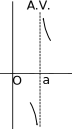
\includegraphics[width=\textwidth]{img-06/asimptota-vertical}	
	\end{minipage}	
	\begin{minipage}{0.7\textwidth}
		Per a cada valor $x=a$ tal que $Q(a)=0$, estudiam la posició relativa calculant els dos límits laterals:
		
		\[ \limx{a^-} \dfrac{P(x)}{Q(x)}=\pm \infty  \qquad\qquad \limx{a^+} \dfrac{P(x)}{Q(x)}=\pm\infty \]	
		
		d'aquesta forma sabem si s'acosta cap a $\pm \infty$ al voltant de l'asímptota vertical.
	\end{minipage}
\end{theorybox}

\begin{mylist}
\exer  \label{exercici:anterior} Determina les asímptotes verticals de les funcions següents:
 
\begin{tasks}(2) 
\task $f(x)=\dfrac{(x+4)\cdot (x-2)}{(x-1)\cdot (x-2)} $  \task  $f(x)=\dfrac{x\cdot (x+4)}{(x-2)\cdot (x-3)} $  
\task  $f(x)=\dfrac{(x+4)^{2} }{(x-1)\cdot (x+4)} $  \task  $f(x)=\dfrac{(x+4)}{(x-1)\cdot (x-3)\cdot (x-5)}$
\end{tasks}

\answers{[$x=1$, $x=2$; $x=3$, $x=1$, $x=1$; $x=3$; $x=5$]}

\addanswersline{}{0}{\mbox{}\par 
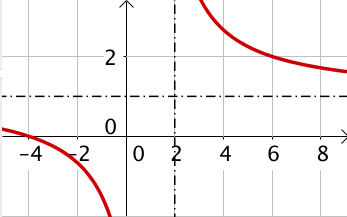
\includegraphics[width=0.21\textwidth]{img-sol/t6-14a}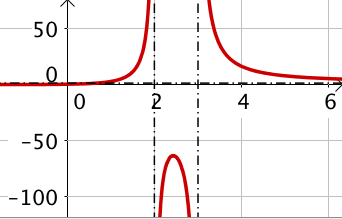
\includegraphics[width=0.21\textwidth]{img-sol/t6-14b}\par
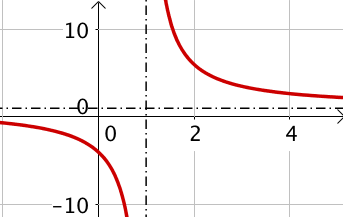
\includegraphics[width=0.21\textwidth]{img-sol/t6-14c}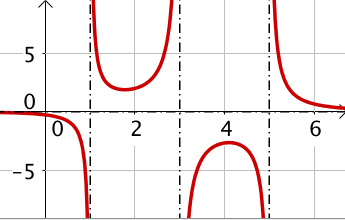
\includegraphics[width=0.21\textwidth]{img-sol/t6-14d}\par
}
\end{mylist}


\subsection{Asímptotes horitzontals}

\begin{theorybox}
	Perquè una funció racional $f(x)=\dfrac{P(x)}{Q(x)}$ tingui una asímptota horitzontal, \newline el grau $P\leq $grau $Q$. L'asímptota és la recta horitzontal $y=L$, essent $L=\limx{\infty }f(x)$.
		\vspace{0.25cm}
	
	\begin{center}
		\textbf{Nota:} Quan grau $P$ $<$ grau $Q$, la recta $y=0$ és l'asímptota horitzontal.
	\end{center}
	\vspace{0.25cm}
	
	\begin{minipage}{0.45\textwidth}
		Per saber si ens acostam per damunt o davall de l'asímptota horitzontal $y=L$ construïm una taula amb dos valors grans (un negatiu i l'altre positiu).
	\end{minipage}
	\begin{minipage}{0.55\textwidth}
		\begin{center}
			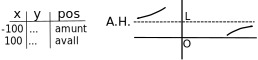
\includegraphics[width=\textwidth]{img-06/asimptota-horitzontal}
		\end{center}
		
	\end{minipage}
	
\end{theorybox}
 

\begin{mylist}
\exer  Determina  les asímptotes horitzontals de les funcions  de l'exercici \ref{exercici:anterior}.

\answers{[$y=1$, $y=3$, $y=1$, $y=0$]}
\end{mylist}
 
 
\pagebreak
 
\subsection{Asímptotes obliqües i branques parabòliques}

\begin{theorybox}
	\video{176}{Asímptotes obliqües}
	Perquè una funció racional $f(x)=\dfrac{P(x)}{Q(x)}$ tingui una asímptota obliqua, el graus han de complir grau $P(x) = $grau $Q(x)+1$. L'equació de l'asímptota obliqua s'obté del quocient de la divisió de $P(x):Q(x)$.
	
	Si es compleix que grau $P(x) > $grau $Q(x)+1$, aleshores la funció creix més ràpidament que una recta, es diu que té branques parabòliques.
\end{theorybox}
\begin{mylist}
\exer  Determina l'asímptota obliqua, si existeix, de cadascuna de les funcions següents:
 \begin{tasks}(2) 
  \task $f(x)=\dfrac{(x+4)\cdot (x-2)}{(x-1)} $ \task  $f(x)=\dfrac{3x^{2} \cdot (x+4)}{(x-2)\cdot (x-3)} $  \task  $f(x)=\dfrac{x^{2} +4}{2(x-1)} $  \task  $f(x)=\dfrac{2x^{2} +4}{x+1} $
\end{tasks}

\answers{[A.O. $y=x+3$, A.O. $y=3x+27$, A.O $y=\frac{x+1}{2}$, A.O. $y=2x-2$]}

\addanswersline{}{0}{
	\mbox{}\par
	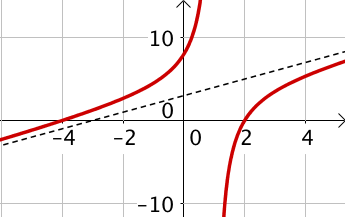
\includegraphics[width=0.21\textwidth]{img-sol/t6-16a}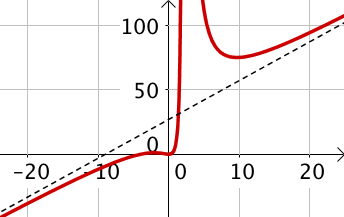
\includegraphics[width=0.21\textwidth]{img-sol/t6-16b}\par 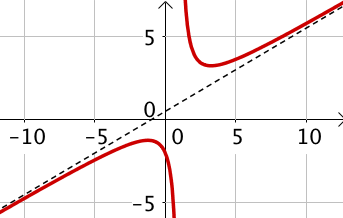
\includegraphics[width=0.21\textwidth]{img-sol/t6-16c} 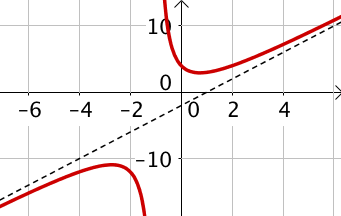
\includegraphics[width=0.21\textwidth]{img-sol/t6-16d}}
 
 \exer  Analitza el comportament a l'infinit de cadascuna de les funcions següents:
 
  \begin{tasks}(3) 
 \task $f(x)=(x+4)^{2} $   \task  $f(x)=\dfrac{3}{(x-2)^{2} } $   \task  $f(x)=\dfrac{x^4+1}{x^2}$  
 %\task  $f(x)=\dfrac{2x^{5} +4}{x+1} $
 \end{tasks}
\answers[cols=1]{[Branques parabòliques a $+\infty$, Asímptota horitzontal $y=0$, Branques parabòliques a $+\infty$, Branques parabòliques a $+\infty$]}
\end{mylist}

\subsection{Calcul d'asímptotes i representació gràfica}

\begin{mylist}
\exer Identifica el tipus d'asímptota i associa cada gràfic amb la seva expressió analítica:

\noindent 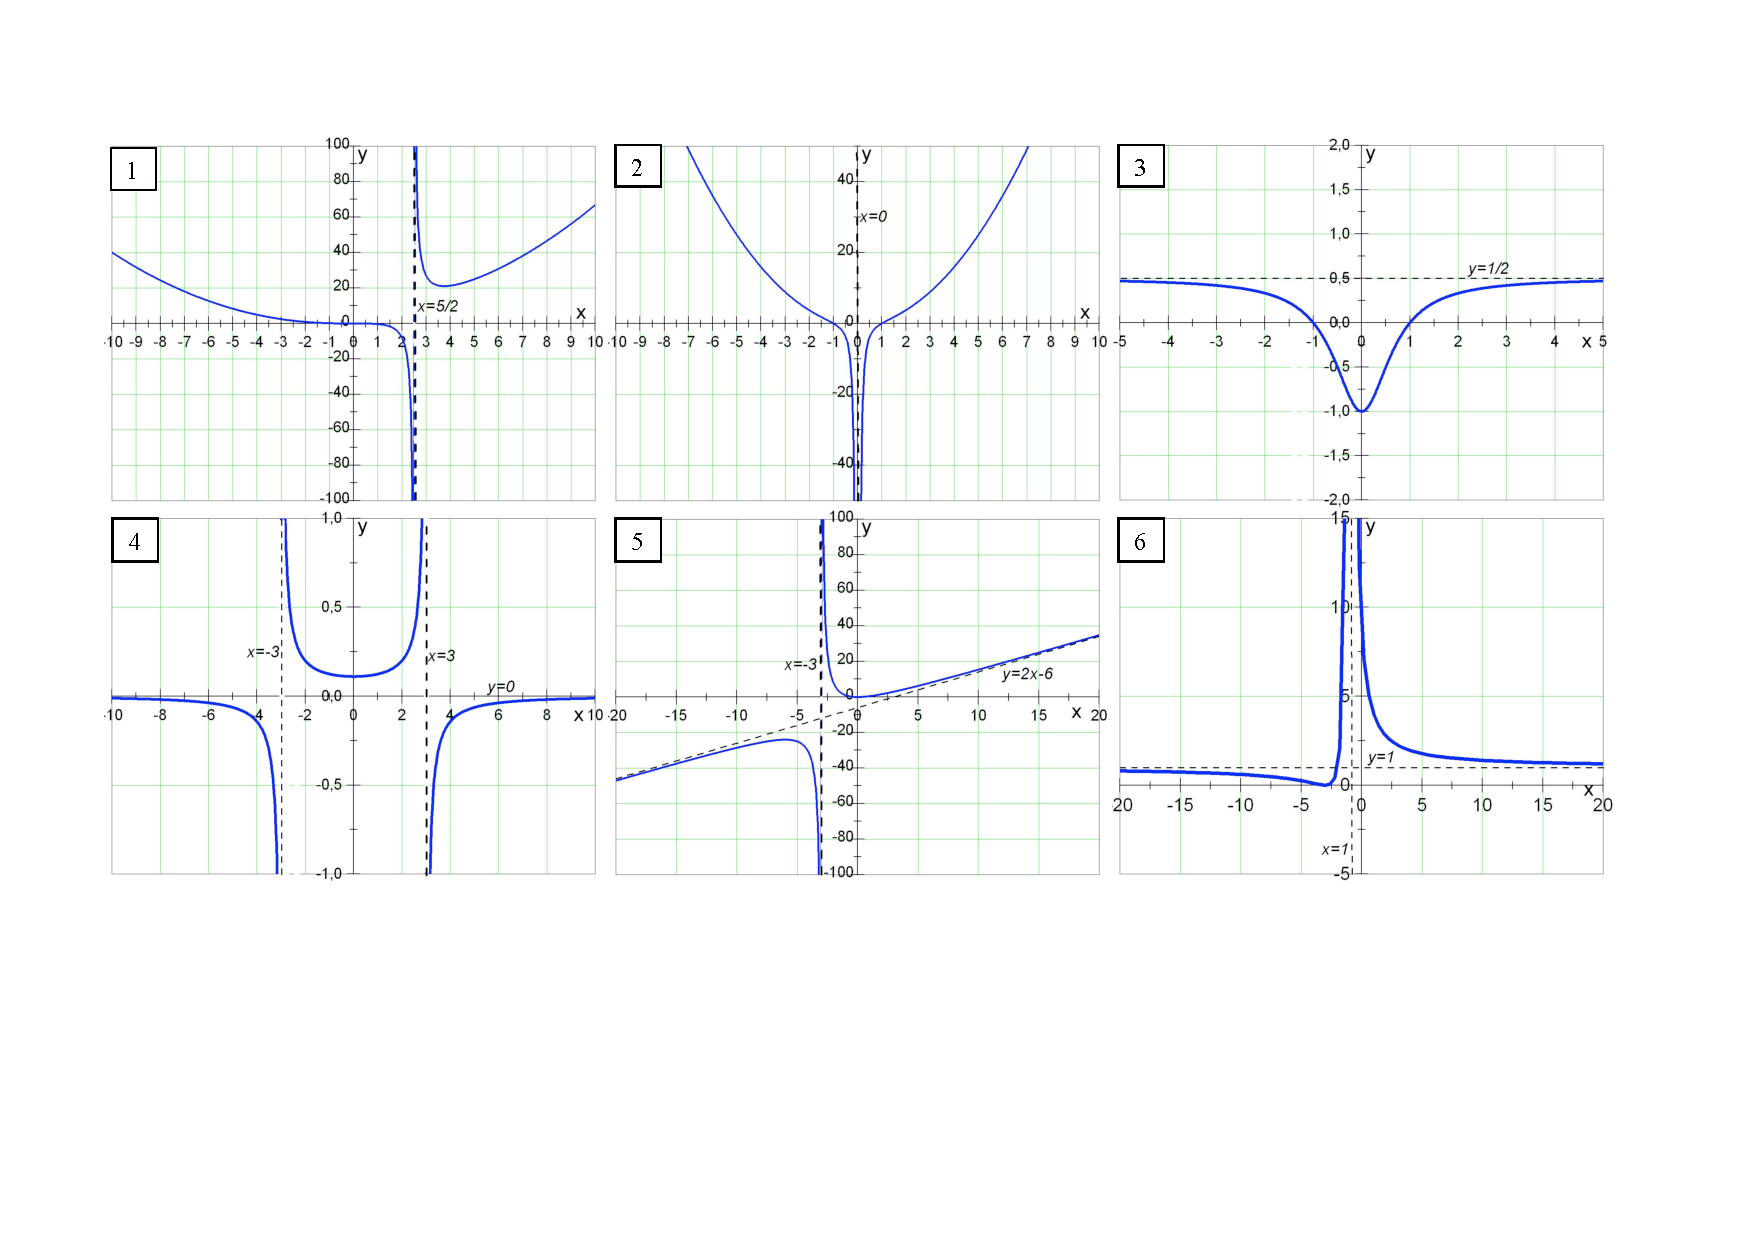
\includegraphics[width=0.92\textwidth]{img-06/misc-asimptotes.pdf} 	

\begin{center}
	\begin{tasks}(3)
		\task $y=\dfrac{x^4-1}{x^2}$
		\task $y=\dfrac{(x+3)^2}{(x+1)^2}$
		\task $y=\dfrac{1}{9-x^2}$
		\task $y=\dfrac{x^2-1}{2x^2+1}$
		\task $y=\dfrac{2x^2}{x+3}$
		\task $y=\dfrac{x^3}{2x-5}$	
	\end{tasks}
\end{center}

\answers{Asímptotes verticals: 1, 2, 4, 5, 6 \par Asímptotes horitzontals: 3, 4, 6 \par
	Asímptotes obliqües: 5 \par Branques parabòliques: 1, 2 \par
	Solució: 1--f; 2--a; 3--d; 4--c; 5--e; 6--b}  

\begin{comment}
\begin{center}
	\begin{tabular}{ll}
		Asímptotes verticals: \makebox[0.2\columnwidth]{\dotfill} & Asímptotes horitzontals: \makebox[0.2\columnwidth]{\dotfill}\\
		Asímptotes obliqües: \makebox[0.2\columnwidth]{\dotfill} & Branques parabòliques: \makebox[0.2\columnwidth]{\dotfill}
	\end{tabular}
\end{center}
 \end{comment}
 
\exer[1] Determina les asímptotes i representa la posició relativa de la funció respecte de les asímptotes: 

\begin{tasks}(2)
	\task   $f(x)=\dfrac{x^{2} -2x}{x-3} $  \task  $f(x)=\dfrac{5}{x^{2} -4} $   \task  $f(x)=\dfrac{x^{2} -5x+6}{x^{2} -4} $ \task  $f(x)=\dfrac{x^{2} -5x}{x^{2} -1} $
	\task  $f(x)=\dfrac{-5x}{(x-1)^{2} } $  \task  $f(x)=\dfrac{-5x^{4} -5}{(x-1)^{2} } $   \task  $f(x)=\ln \dfrac{5x}{(x-1)^{2} } $  \task  $f(x)=\sqrt{\dfrac{5x}{(x-1)^{2} } } $
\end{tasks}
\answers[cols=1]{[AV. $x=3$ AO. $y=x+1$, 	AV. $x=\pm 2$ AH. $y=0$, 	AV. $x=- 2$ AH.  $y=1$,  		AV. $x=\pm 1$ AH.  $y=1$, 	AV. $x=1$ AH.  $y=0$,  AV. $x=1$ BP., AV. $x=0$ i $x=1$ BP., AV. $x=1$ AH. $y=0$]}
 

\end{mylist} 
 
 
\section{Continuïtat de funcions}

\begin{theorybox}[Tipus de discontinuïtats]
Existeixen 4 motius pels quals una funció pot ser discontínua en un punt $x=a$:
\begin{enumerate}
	\item \textbf{Salt infinit o discontinuïtat asimptòtica:} La funció presenta una asímptota en $x=a$
	\item \textbf{De salt finit:} La funció presenta un bot
	\item \textbf{Li falta un punt:} No es pot calcular el valor de la funció a $x=a$
	\item \textbf{Punt desplaçat:} Aquest cas, el punt existeix però es troba a una altura incorrecta.
\end{enumerate}

Els casos 3, 4 s'anomenen \textbf{discontinuïtats evitables.}

\begin{center}
	\fbox{
	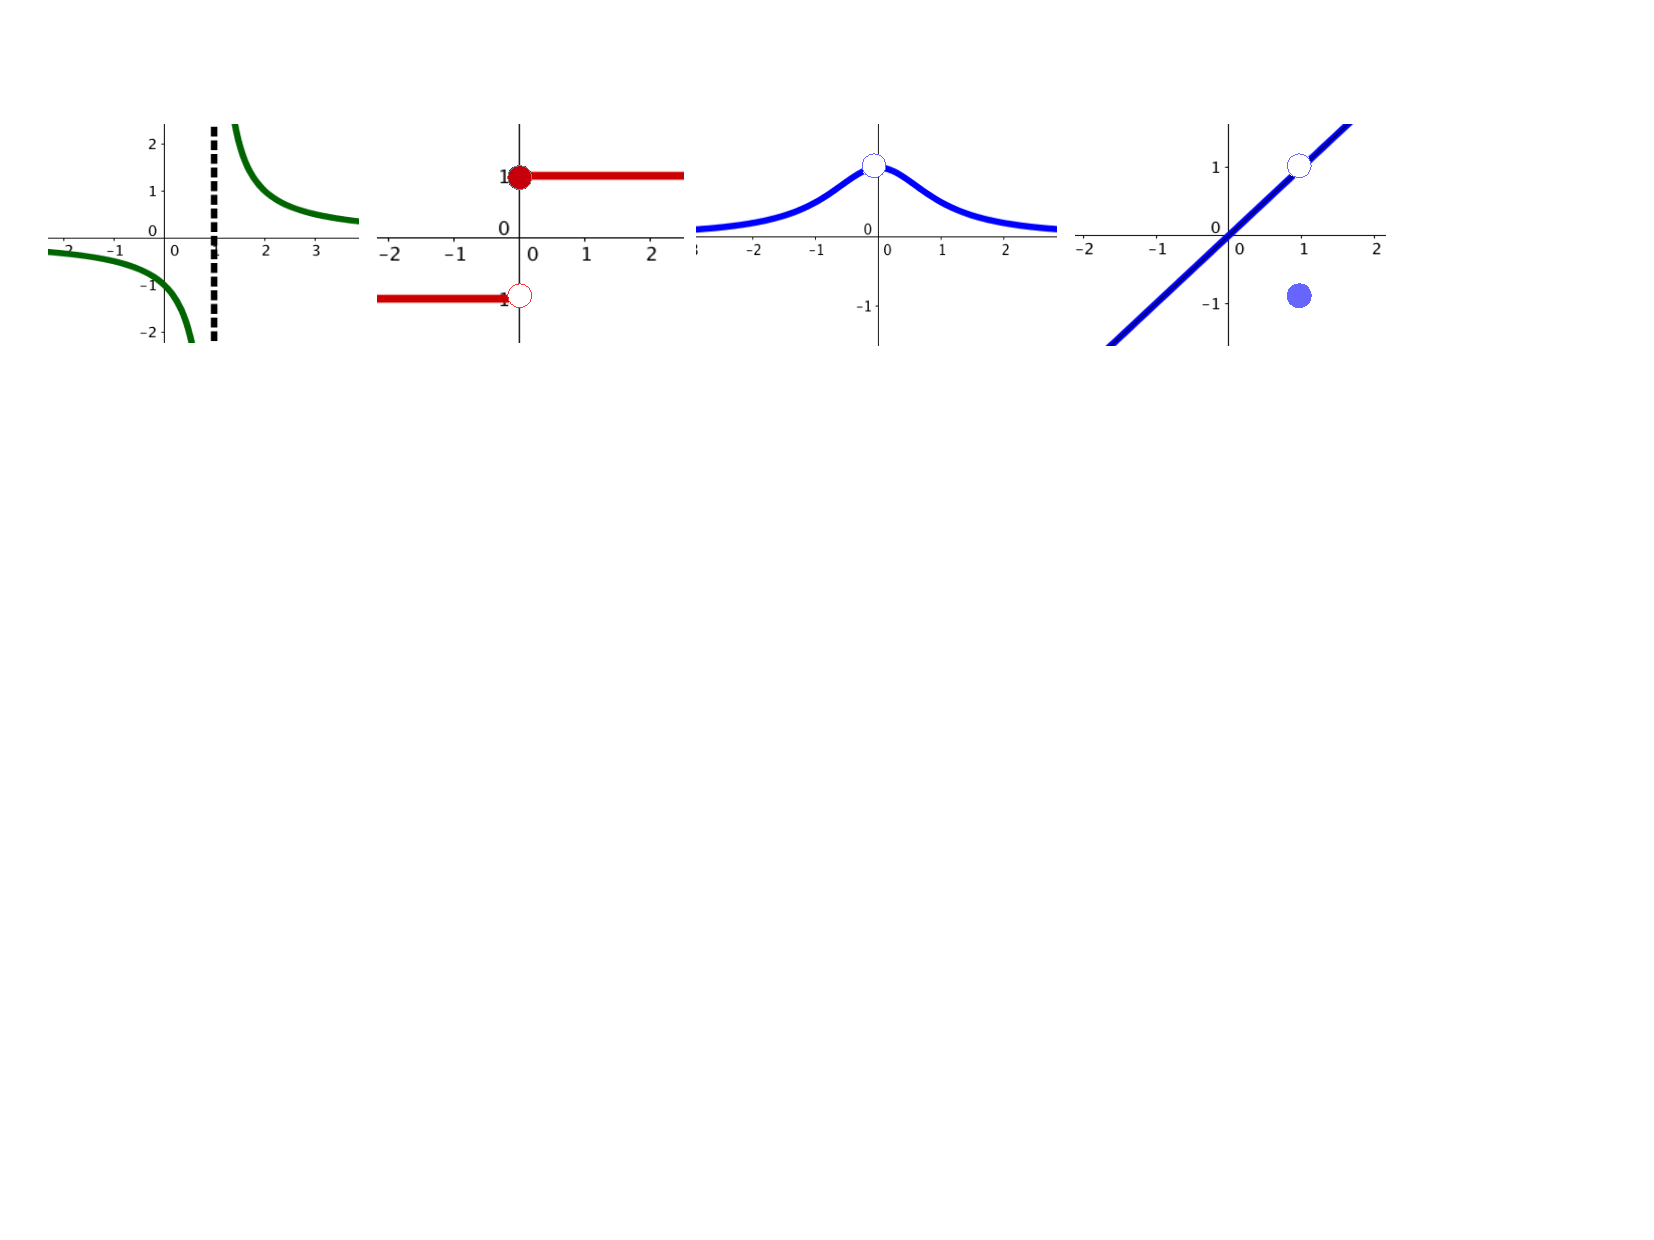
\includegraphics[width=0.93\textwidth]{img-06/chap-fe-tipusdiscont}
}
\end{center}
\end{theorybox}
 
\begin{theorybox}[Funció contínua en un punt]
	Per a que una funció sigui contínua en un punt $x=a$ s'ha de complir:
	\begin{enumerate}
		\item \makebox[7.5cm][l]{Els límits $\limx{a^\pm} f(x)$ han d'ésser finits} (Evitam asímptotes)
		\item \makebox[7.5cm][l]{$\limx{a^-} f(x) = \limx{a^+} f(x) = \limx{a} f(x)$}  (Evitam salts)
		\item \makebox[7.5cm][l]{Existeix $f(a)$]} (Evitam li falta un punt)
		\item \makebox[7.5cm][l]{$\limx{a} f(x)=f(a)$} (Evitam punt desplaçat)
	\end{enumerate}
	Una funció és diu que és contínua si és contínua en tots els punts del seu domini. 
\end{theorybox}

\pagebreak

\begin{mylist}
	\exer Estudia la continuïtat de les funcions següents:
	\begin{tasks}(2)
	\task   $f(x)=\dfrac{x+1}{x^{2} -1} $   \task  $f(x)=\sqrt{x-5} $  \task  $f(x)=\log _{2} (x-3)$  \task  $f(x)=\left\{\begin{array}{cc} {2+x^{2} } & {si\; x\le 0} \\ {1+e^{x} } & {si\; x>0} \end{array}\right. $
	\end{tasks}
\answers[cols=1]{[$x=-1$ li falta un punt; $x=1$ asímptota vertical, És continua a $[5,+\infty)$, És continua a $(3,+\infty)$, És contínua a $\Re$]}

	\exer  Estudia la continuïtat de les funcions següents: 
	\begin{tasks}(2)
	\task   $f(x)=\left\{\begin{array}{ccc} {-2x+3} & {si} & {x<-1} \\ {2+x^{2} } & {si} & {-1\le x\le 1} \\ {\dfrac{3}{x} } & {si} & {x>1} \end{array}\right. $   \startnewitemline  \task  $f(x)=x-\sqrt{x-2} $ \task $f(x)=\left|x-3\right|-1$
    \end{tasks}
	\answers[cols=1]{[Té una discontinuïtat de salt finit a $x=-1$, És continua a $[2,+\infty)$, És contínua a $\Re$]}
	
	\exer Estudia la continuïtat de les funcions següents, indicant en cada cas el tipus de discontinuïtat. Representa-les gràficament.
\begin{tasks}(2)
	\task $f(x)=\left\{\begin{array}{c} {3^{x} \quad \quad x<-2} \\ {4-x^{2} \quad -2\le x\le 1} \\ {\log _{2} x\quad \quad x>1} \end{array}\right. $  \task $g(x)=\left\{\begin{array}{c} {\dfrac{1}{x} \quad \quad x<0} \\ {x^{2} -3x\quad 0\le x<3} \\ {\sqrt{x-3} \quad \quad x\ge 3} \end{array}\right. $   \task  $h(x)=\left|x^{2} -5x\right|$
\end{tasks}
\answers[cols=1]{[Té discontinuïtats de salt a $x=-2$ i $x=1$, Té discontinuïtat asimptòtica a $x=0$, És contínua a $\Re$ ]}

\addanswersline{}{0}{\mbox{} \par
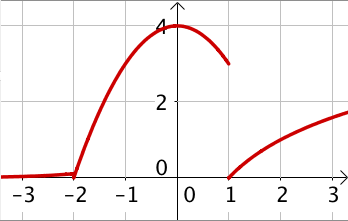
\includegraphics[width=0.21\textwidth]{img-sol/t6-22a}
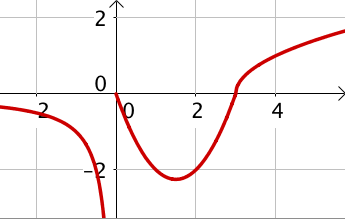
\includegraphics[width=0.21\textwidth]{img-sol/t6-22b} \par 
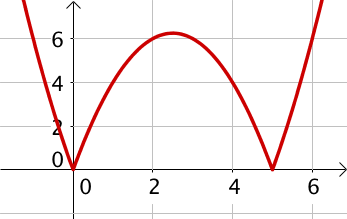
\includegraphics[width=0.24\textwidth]{img-sol/t6-22c}
}
	
	\exer Estudia la continuïtat de les funcions següents, indicant en cada cas el tipus de discontinuïtat.
	\begin{tasks}(3)
	\task  $f(x)=\left|x^{2} -25\right|$   \task  $g(x)=2-\dfrac{\left|x\right|}{x} $    \task $h(x)=\dfrac{x^{2} -2\left|x\right|}{x-3} $
	\end{tasks}
\answers[cols=1]{[Contínua a $\Re$, Salt finit a $x=0$, Té asímptota a $x=3$]}
	
%	\exer Estudia la continuïtat de les funcions següents, indicant en cada cas el tipus de discontinuïtat.  
%	\begin{tasks}(3)
%	\task $f(x)=\dfrac{3x+5}{x^{2} -4x+3} $  \task $g(x)=\dfrac{7x+2}{x^{2} +x} $   \task $h(x)=\dfrac{x^{2} -5x+4}{x^{2} -2x-3} $
%	\end{tasks}
	
	\exer Estudia la continuïtat de les funcions següents, indicant en cada cas el tipus de discontinuïtat. 
	\begin{tasks}(3)
	\task $f(x)=\sqrt{x^{2} -x-6} $  \task $g(x)=\sqrt{\dfrac{2-x}{x^{2} -4} } $   \task $h(x)=\sqrt{\dfrac{3-x}{x^{2} -3x} }$
	\end{tasks}
	\answers[cols=1]{[Contínua en domini $(-\infty,-2)\cup(3,+\infty)$, Contínua en domini $(-\infty,-2)$; A.V. a $x=-2$, Contínua en domini $(-\infty,0)$;  A.V. a $x=0$]}
	
	\exer Estudia la continuïtat de les funcions següents, indicant en cada cas el tipus de discontinuïtat. 
	\begin{tasks}(2)
	 \task $f(x)=\ln \left(\dfrac{4-x}{x-5} \right)$ 
	 \task  $g(x)=\ln \left(-x^{2} -x+2\right)$ 
	 %\task $h(x)=\ln \left(\dfrac{9-x^{2} }{\left(x-3\right)^{2} } \right)$
	%
	 \task $h(x)=e^{\frac{x^{2} -9}{7+x} } $   
	 \task  $i(x)=e^{\sqrt{x-5} } $  
	% \task  $h(x)=2^{\frac{\sqrt{x-1} }{x^{2} -1} } $
	\end{tasks}
\answers[cols=1]{[Domini $(4,5)$. A.V. a $x=4$ i $x=5$, Domini $(-2,1)$. A.V. a $x=-2$ i $x=1$, A.V. $x=-7$, Contínua a $[5,+\infty]$]}
	
	\exer Donada la funció $f(x)=\left\{\begin{array}{cc} {3-x^{2} } & {x<0} \\ {2+e^{x} } & {x\ge 0} \end{array}\right. $.  a) Estudia la seva continuïtat. b) Representa la seva gràfica. 
\answers[cols=1]{És contínua a $\Re$.\par 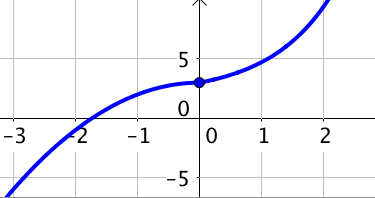
\includegraphics[width=0.4\textwidth]{img-sol/t6-28}}	

	\exer Donada la funció $f(x)=\left\{\begin{array}{c} {x-3} \\ {x^{2} -5} \\ {\dfrac{2}{x} } \end{array}\begin{array}{c} {x<-1} \\ {\; \; -1\le x<1} \\ {x\ge 1} \end{array}\right. $.  a) Estudia la seva continuïtat. b) Representa la seva gràfica. 
\answers[cols=1]{Continua excepte $x=1$ salt finit.\par 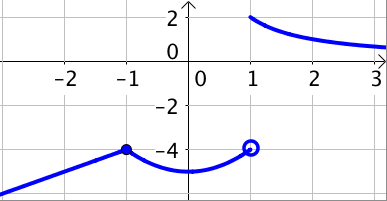
\includegraphics[width=0.4\textwidth]{img-sol/t6-29}}	
	
%	\exer Donada la funció $f(x)=\left\{\begin{array}{cc} {4-x^{2} } & {x<2} \\ {x^{2} -4} & {x\ge 2} \end{array}\right. $.  a) Estudia la seva continuïtat. b) Representa la seva gràfica.
	
	
	\exer Esbossa la gràfica de la funció $f(x)=\dfrac{x}{x^{2} -25} $ indicant les seves asímptotes i els seus punts de discontinuïtat.
	
	\answers{A.V. $x=\pm 5$; A.H. $y=0$. És discontinua degut les asímptotes a $x=\pm 5$.\par 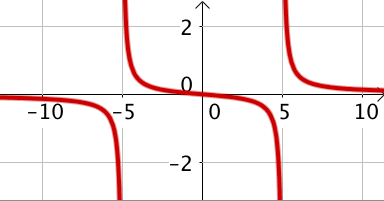
\includegraphics[width=0.4\textwidth]{img-sol/t6-31} }
 


\end{mylist}

	\subsection{Discussió de la continuïtat en funció d'un paràmetre}
	
 
	\begin{resolt}[E]{Determina el valor de $k$ perquè la funció $f(x)=\left\{\begin{array}{cc} {2-x^{2} } & {si\; x\le 1} \\ {k+x} & {si\; x>1} \end{array}\right. $ sigui contínua en tota la recta real.
		}
		Donat que el primer tros és una paràbola i el segon tros una línia recta, cada funció per separat és contínua. L'únic que hem d'imposar és que sigui contínua en el punt d'unió $x=1$ de la funció a trossos. \vspace{0.25cm}
		
		Estudiam la continuïtat en el punt $x=1$:
		\begin{enumerate}
			\item Els límits laterals són finits; no té asímptotes \vspace{0.25cm}
			
			\item $\limx{1^-} f(x)=\limx{1^-} 2-x^2 = 2-1^2 = 1$ i  \vspace{0.25cm}
			
			$\limx{1^+} f(x)=\limx{1^+} k+x = k+1$. \vspace{0.25cm}
			
			Si imposam que els dos límits laterals siguin iguals, \par $1=1+k$ ens duu al resultat $k=0$.
			\vspace{0.25cm}
			
			\item Existeix $f(1)=1$ \vspace{0.25cm}
			\item També es compleix que $\limx{1} f(x)=f(1)=1$. 
		\end{enumerate}
		La resposta és que $k=0$.
	\end{resolt}
	\vspace{0.5cm}

\begin{mylist}		
	\exer Donada la funció $f(x)=\left\{\begin{array}{cc} {3-x^{2} } & {x<2} \\ {k+x} & {x\ge 2} \end{array}\right. $.  a) Determina el valor de  $k$ perquè la funció sigui contínua en tota la recta real. b) Representa la seva gràfica 
	
	\answers{$k=-3$; \ggblink{https://www.geogebra.org/m/PS5YUdBN}}
	
	\exer Calcula $k$ perquè la funció $f(x)=\left\{ \begin{array}{ll}
	\dfrac{x^2-1}{x-1}  & x \neq 1 \\
	k & x = 1
	\end{array} \right.$ sigui contínua.
	
	\answers{$k=2$; \ggblink{https://www.geogebra.org/m/K6YYNbCC}}
	 
	\exer En la funció $f(x)=\left\{ \begin{array}{ll}
	\dfrac{px+1}{x-4}  & x \leq 1 \\
	\dfrac{x-1}{x^2-x} & x > 1
	\end{array} \right.$
	a) Troba el valor de $p$ perquè sigui contínua en $x=1$. b) Hi ha algun altre punt en què sigui discontínua?
	
	\answers{ $p=-4$; \ggblink{https://www.geogebra.org/m/mU2vFjBH}.\par No és discontínua en cap altre punt.}
 	
	\exer Estudia la continuïtat de la funció $f(x)=\left\{ \begin{array}{ll}
		3-ax^2  & x \leq 1 \\
	\dfrac{2}{ax} & x > 1
	\end{array} \right.$ segons el valor del paràmetre $a$.

	\answers{ Si $a=1$, la funció és contínua; Si $a\neq 1$, la funció presenta un salt finit a $x=1$.  \ggblink{https://www.geogebra.org/m/KCtQrh29} }

	\exer[-1] Estudia la continuïtat de la funció $f(x)=\left\{ \begin{array}{ll}
	x^2  & x \leq a \\
	a+2 & x > a
	\end{array} \right.$ segons el valor del paràmetre $a$.
	\answers{Has d'imposar les condicions de continuïtat en $x=a$; obtindràs l'equació de segon grau $a^2-a-2=0$. Per a $a=-1$ i $a=2$ és continua; discontinuïtat de salt.}	
	
	\addanswersline{}{0}{ \ggblink{https://www.geogebra.org/m/n5pZEvVR} }
 

	\exer Determina $a$ i $b$ perquè la funció $f(x)=\left\{ \begin{array}{ll}
	\ln x  & 0 < x \leq 1 \\
	a x^2 +b & x > 1
	\end{array} \right.$ sigui contínua i compleixi que $f(2)=3$.

	\answers{$a=1$ i $b=-1$}
	
\end{mylist}

 \vspace{0.25cm}
\begin{autoaval}{32}
\begin{mylist}
	
	%\answers{\textbf{--10.} Autoavaluació: 1a; 2a; 3c; 4a; 5a; 6c; 7a; 8d; 9c; 10b}
	
	\exer[2] Calcula el límit $\limx{1} \left(\dfrac{1}{x^{2} -1} -\dfrac{1}{x-1} \right)$.
	
	%\begin{tasks}(4)
	%\task $\infty$  \task 0   \task 1   \task 2/3
	%\end{tasks}
	\answers{$\limx{1^-} f=+\infty$, $\limx{1^+} f=-\infty$}
	
	\exer[2] Calcula el límit $\limx{-2} (x^{2} -x-2)\cdot \left(\dfrac{1}{x+2} \right)$.
	%\begin{tasks}(4)
	%\task $\infty$  \task 0   \task 1  \task $-$1
	%\end{tasks}
	\answers{$\limx{-2^-} f=-\infty$, $\limx{-2^+} f=+\infty$}

	\exer[2] Calcula el límit $\limx{1} \left(\dfrac{x^{2} -4x+3}{x^{2} +x-2} \right)$.
	%\begin{tasks}(4)
	%\task $\infty$  \task0  \task $-$2/3  \task %$-$1
	%\end{tasks}
	\answers{$-2/3$}
	
	\exer[2] Calcula el límit $\limx{-1} \dfrac{\sqrt{2+x} -1}{x+1} $
	%\begin{tasks}(4)
	%\task 1/2   \task 0  \task $-$$\infty$  \task %$-$1
	%\end{tasks}
	\answers{$1/2$}
	
 
		
		\exer[2] Calcula els límits a) $\limx{\infty } \dfrac{5x^{3} +7x-4}{x^{3} +3}$ \quad b) $\limx{\infty } \dfrac{5x^{3} +7x-4}{x^{2} +3}$  
		%\begin{tasks}(4)
		%\task $\infty$  \task 0   \task 5   \task 1
		%\end{tasks}
		\answers{a) $5$, b) $+\infty$}
		


	\exer[2] Calcula el límit $\limx{\infty } \left(\dfrac{3x+1}{3x-2} \right)^{2x^{2} +1} $ 
	%\begin{tasks}(4)
	%\task $\infty$  \task 0   \task 5   \task 1
	%\end{tasks}
	\answers{$\infty$}
 

	\exer[2] Estudia la continuïtat de $f(x)=\left\{\begin{array}{cc} {\dfrac{x^{3} -3}{x} } & {si\; x<0} \\ {3x+2} & {si\; x\ge 0} \end{array}\right. $  en $x=0$. 
\answers{Té un salt infinit a $x=0$}

	\exer[2] Estudia la continuïtat de $f(x)=\left\{\begin{array}{cc} {x^{3} -3} & {si\; x<2} \\ {3x+2} & {si\; x\ge 2} \end{array}\right. $  en $x=2$.  
\answers{Té un salt finit a $x=2$}

	\exer[2] Troba  el valor de $k$ perquè $f(x)=\left\{\begin{array}{cc} {x^{3} } & {si\; x<2} \\ {3x+k} & {si\; x>2} \end{array}\right. $  sigui contínua en $x=2$. 
	\answers{$k=2$}
\end{mylist}
\end{autoaval}
 
 \newpage
 
\resum
\begin{center}
	\setlength\LTleft{0pt}
	\setlength\LTright{0pt}
	\ftimes{10.5}{11}
	\fontsize{10.5}{11}
	\renewcommand{\arraystretch}{2}
	\begin{longtable}[h]{|>{\raggedleft\arraybackslash}p{0.19\textwidth}|p{0.77\textwidth}|}
		\hline %inserts double horizontal lines
		\rowcolor{lightgray}
		
		\textbf{Apartat} & \textbf{Resum} \\   [0.5ex] 
		\hline
		
		\begin{comment}
		\cellcolor{lightgray}\noindent \textbf{ Definició de límit }  &    
		\begin{minipage}{0.52\textwidth}
		$\mathop{\lim}\limits_{a} f(x)=L$ $\Leftrightarrow$ Per tot $\epsilon$ $>$ 0, existeix un $\delta$ $>$ 0 tal que, sempre que $|x-a|<\delta$, 
		
		es compleix $|f(x)-L|<\epsilon$.
		\end{minipage}
		\begin{minipage}{4cm}
		\includegraphics*[width=3.5cm]{img-06/deflim}
		\end{minipage}
		\\
		\hline
		\end{comment}
		
		\cellcolor{lightgray}\textbf{ Límit lateral per la dreta }  &    
		$\mathop{\lim}\limits_{x \to a^{+} } f(x)=L$ el valor de $f(x)$ tendeix a L quan $x$ tendeix a $a$, sempre que es compleixi $x>a$
		\sample{
			La funció $f(x)=\left\{\begin{array}{cc} {x^{3} } & {si\; x<2} \\ {3x+2} & {si\; x\ge 2} \end{array}\right. $ 
			
			té lateral per la dreta  8, ja que $\limx{x \to 2^+} x^{3} =2^{3} =8$}
		\hline
		
		\cellcolor{lightgray}\textbf{Límit lateral per l'esquerra}  &    
		$\mathop{\lim}\limits_{x \to a^{-} } f(x)=L$ si  el valor $f(x)$ tendeix a $L$ quan $x$ tendeix a $a$, sempre que es compleixi la condició $x<a$. \\ \hline
		
		\cellcolor{lightgray}\textbf{ Existència del límit }  &    
		
		El límit existeix si els dos límits laterals són iguals
		
		$\mathop{\lim}\limits_{x \to a} f(x)=\mathop{\lim}\limits_{x \to a^{+} } f(x)=\mathop{\lim}\limits_{x \to a^{-} } f(x)=L$  
		
		\begin{comment}
		\sample{
		La funció $f(x)=\left\{\begin{array}{cc} {x^{3} } & {si\; x<2} \\ {3x+2} & {si\; x\ge 2} \end{array}\right.$ té límit en \textit{x} = 2 
		}
		\end{comment}
		\\ \hline
		
		\cellcolor{lightgray}\noindent \textbf{Asímptotes  }  &    
		Si $\mathop{\lim}\limits_{x \to +\infty } f(x)=K$ hi ha una asímptota horitzontal $y=K$.
		
		Si $\mathop{\lim}\limits_{x \to a} f(x)=\infty $ hi ha una asímptota vertical a $x=a$.
		\sample{
			$f(x)=\dfrac{2x+1}{x-1} $ té asímptota horitzontal $y=2$ i asímptota vertical $x=1$.
		} 
		\hline 
		
		\begin{comment}
		\cellcolor{lightgray}\noindent \textbf{Propietats dels límits  }  &    
		$\mathop{\lim}\limits_{a} (f(x)+g(x))=\mathop{\lim}\limits_{a} f(x)+\mathop{\lim}\limits_{a} g(x)$\newline $\mathop{\lim}\limits_{a} (f(x)\cdot g(x))=\mathop{\lim}\limits_{a} f(x)\cdot \mathop{\lim}\limits_{a} g(x)$\newline $\mathop{\lim}\limits_{a} (K\cdot f(x))=K\cdot \mathop{\lim}\limits_{a} f(x)$\newline $\mathop{\lim}\limits_{a} (\dfrac{f(x)}{g(x)} )=\dfrac{\mathop{\lim}\limits_{a} f(x)}{\mathop{\lim}\limits_{a} g(x)} $ si $g(a)\neq 0$.
		\\
		\hline
		\end{comment}
		
		\cellcolor{lightgray}  \textbf{Continuïtat d'una funció en un punt  }  &    
		Una funció $f(x)$ és contínua en el punt $x=a$, si es compleixen:
		\begin{enumerate}
			\exer Els límits $\mathop{\lim}\limits_{x \to a^{\pm}} f(x)$ són finits
			\exer Existeix el limit $\mathop{\lim}\limits_{x \to a^+} f(x)=\mathop{\lim}\limits_{x \to a^+} f(x)=\mathop{\lim}\limits_{x \to a} f(x)$.
			\exer Existeix $f(a)$
			\exer El límit i la funció coincideixen $\mathop{\lim}\limits_{x \to a} f(x) = f(a)$
		\end{enumerate}
		La condició 1. assegura que no hi ha asímptotes verticals. La condició 2. significa que no hi ha salts finits. La condició 3. vol dir que no falten punts i finalment 4. assegura que no hi ha punts desplaçats.
		\begin{comment}
		\sample{
		La funció $f(x)=\left\{\begin{array}{cc} {x^{3} } & {si\; x<2} \\ {3x+2} & {si\; x\ge 2} \end{array}\right. $ és contínua en $x=2$.
		}
		\end{comment}
		\\ \hline
		
		\begin{comment}
		\cellcolor{lightgray}\noindent \textbf{Propietats de les funcions contínues }  &    
		La suma i el producte de funcions contínues és una funció contínua.\newline El quocient de funcions contínues és una funció contínua si no s'anul·la el denominador.
		\sample{
		Els polinomis són funcions contínues en $\Re$\newline $f(x)=\dfrac{1}{x} $ és contínua en $\Re$ $-$ $\{$0$\}$ 
		}
		\hline
		\end{comment}
		
		\cellcolor{lightgray}\noindent \textbf{ Tipus de discontinuïtats }  &    
		Asímptòtica o salt infinit; De salt finit; Evitables: Li falta un punt, i té un punt desplaçat.
		\sample{
			$f(x)=\left\{\begin{array}{cc} {x^{3} } & {si\; x<2} \\ {3x+2} & {si\; x>2} \end{array}\right. $ evitable (li falta un punt) en \textit{x} = 2\newline $f(x)=\dfrac{1}{x} $ té un salt infinit en $x=0$
		}
		\hline 
	\end{longtable}
\end{center}
 